\documentclass[tikz,border=10pt]{standalone}
\usepackage{tikz}
\usetikzlibrary{arrows.meta,positioning,calc,backgrounds,fit,shapes.geometric}
\usepackage[scaled=0.92]{helvet}
\renewcommand{\familydefault}{\sfdefault}
\usepackage{amsmath,amssymb}
\definecolor{ink}{HTML}{262624}
\definecolor{mute}{HTML}{8A8984}
\definecolor{line}{HTML}{BDBBB5}
\definecolor{acc}{HTML}{2A78D6}
\definecolor{accbg}{HTML}{F1F6FD}
\tikzset{
  >={Latex[length=2.2mm]},
  every node/.style={text=ink},
  b/.style={draw=line, fill=white, rounded corners=2pt, align=center, inner sep=6pt,
            minimum height=10mm, text width=#1, font=\small},
  b/.default=40mm,
  a/.style={b=#1, draw=acc, fill=accbg},
  a/.default=40mm,
  t/.style={font=\footnotesize, text=mute, align=center},
  e/.style={->, draw=mute, line width=0.6pt},
  ea/.style={->, draw=acc, line width=0.9pt},
  eh/.style={->, draw=acc, line width=0.9pt, dash pattern=on 3pt off 2pt},
}

\begin{document}
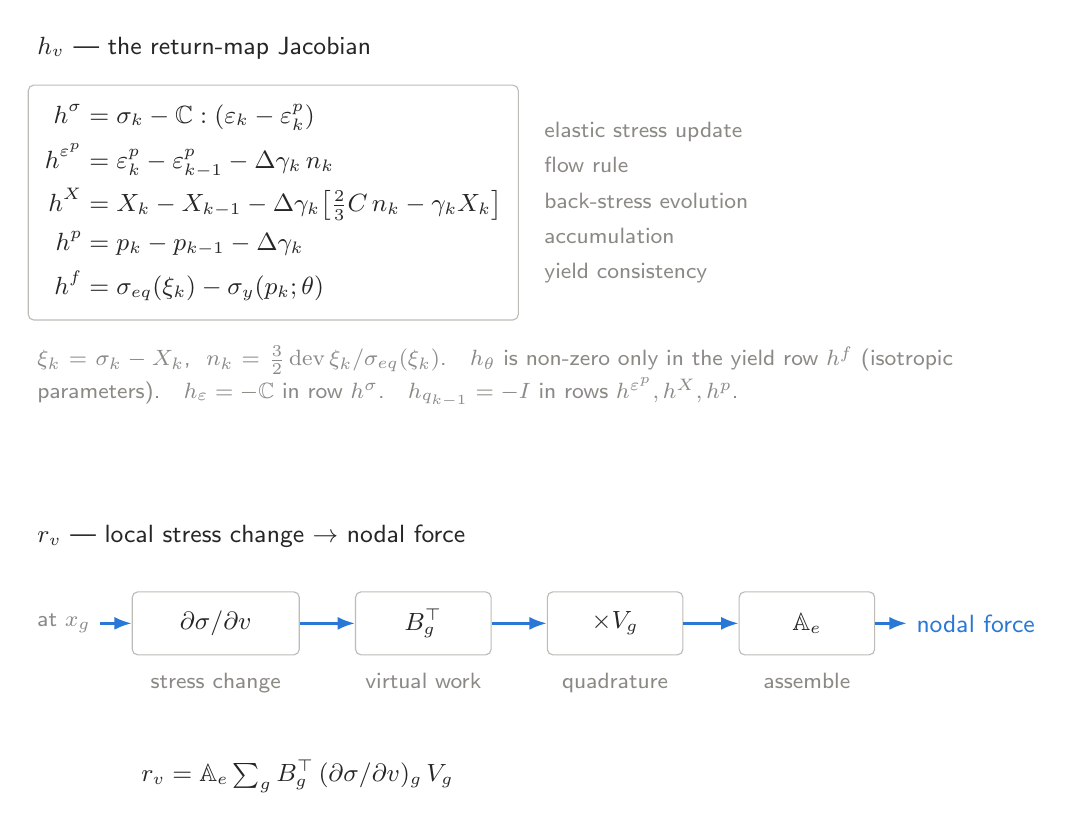
\begin{tikzpicture}
% (1) local Jacobian
\node[anchor=north west, font=\small\bfseries] (t1) at (0,0) {$h_v$ \textmd{--- the return-map Jacobian}};
\node[below=2mm of t1.south west, anchor=north west, draw=line, rounded corners=2pt, inner sep=6pt, font=\small] (H) {%
$\begin{aligned}
h^{\sigma} &= \sigma_k - \mathbb C:(\varepsilon_k-\varepsilon^p_k)\\
h^{\varepsilon^p} &= \varepsilon^p_k-\varepsilon^p_{k-1}-\Delta\gamma_k\, n_k\\
h^{X} &= X_k - X_{k-1} - \Delta\gamma_k\big[\tfrac23 C\, n_k - \gamma_k X_k\big]\\
h^{p} &= p_k - p_{k-1} - \Delta\gamma_k\\
h^{f} &= \sigma_{eq}(\xi_k) - \sigma_y(p_k;\theta)
\end{aligned}$};
\node[right=2mm of H, t, align=left] {elastic stress update\\[3.2pt] flow rule\\[3.2pt] back-stress evolution\\[3.2pt] accumulation\\[3.2pt] yield consistency};
\node[below=2mm of H.south west, anchor=north west, t, align=left, text width=118mm] {%
$\xi_k=\sigma_k-X_k$,\ \ $n_k=\tfrac32\,\mathrm{dev}\,\xi_k/\sigma_{eq}(\xi_k)$.\quad
$h_\theta$ is non-zero only in the yield row $h^f$ (isotropic parameters).\quad
$h_\varepsilon=-\mathbb C$ in row $h^\sigma$.\quad $h_{q_{k-1}}=-I$ in rows $h^{\varepsilon^p}, h^X, h^p$.};
% (2) r_v
\begin{scope}[shift={(0,-62mm)}]
\node[anchor=north west, font=\small\bfseries] (t2) at (0,0) {$r_v$ \textmd{--- local stress change $\to$ nodal force}};
\node[below=6mm of t2.south west, anchor=north west, t] (x) {at $x_g$};
\node[b=17mm, right=4mm of x, minimum height=8mm] (a1) {$\partial\sigma/\partial v$};
\node[b=13mm, right=7mm of a1, minimum height=8mm] (a2) {$B_g^{\top}$};
\node[b=13mm, right=7mm of a2, minimum height=8mm] (a3) {$\times V_g$};
\node[b=13mm, right=7mm of a3, minimum height=8mm] (a4) {$\mathbb A_e$};
\node[right=4mm of a4, font=\small, text=acc] (o) {nodal force};
\foreach \u/\v in {x/a1,a1/a2,a2/a3,a3/a4,a4/o} \draw[ea] (\u) -- (\v);
\node[below=1mm of a1, t] {stress change}; \node[below=1mm of a2, t] {virtual work};
\node[below=1mm of a3, t] {quadrature}; \node[below=1mm of a4, t] {assemble};
\node[below=12mm of a1.south west, anchor=north west, font=\small] {$r_v = \mathbb A_e \sum_g B_g^{\top}\,(\partial\sigma/\partial v)_g\,V_g$};
\end{scope}
\end{tikzpicture}
\end{document}
